\section{环境与工具}
\subsection{Linux操作系统}
\subsubsection{什么是操作系统}
现代计算机由一个或多个处理器、主存、磁盘以及各种输入输出设备组成。操作系统是管理这些组件,并将硬件抽象为统一软件接口的一层软件。
\subsubsection{用户和用户组}
Linux系统是多用户多任务的分时操作系统。根用户账号是\mintinline{bash}{root},拥有最高管理权限,为系统安全通常不直接使用根用户登录。每个用户都属于一个用户组,系统可对用户组中的用户进行集中管理。

\subsubsection{文件和目录权限}
在Linux中,文件和目录具有访问权限。每个文件包含九个权限位,分别定义所有者、所有者所在用户组和其他用户的访问权限。
\begin{minted}{bash}
-rwxr--r-- 1 user user 54130 Jan 8 12:14 README.md
\end{minted}
最前面的 \mintinline{bash}{-} 表示文件,\mintinline{bash}{d} 表示目录,\mintinline{bash}{l} 表示符号链接,后面九位每三位为分隔,\mintinline{bash}{r} 表示读取,\mintinline{bash}{w} 表示写入,\mintinline{bash}{x} 表示执行,\mintinline{bash}{-} 表示无权限。


\subsubsection{文件和目录操作命令}
\begin{enumerate}[label=\arabic*.]
    \item \textbf{\mintinline{bash}{ls}命令}:用于列出指定目录下的子目录及文件名称,格式为\mintinline{bash}{ls [选项] 路径},如\mintinline{bash}{ls -a}可连同隐藏文件一起列出,\mintinline{bash}{ls -l}可列出文件和目录的属性与权限等详细数据。
    \item \textbf{\mintinline{bash}{cd} 命令}:改变当前工作目录,格式为\mintinline{bash}{cd 路径}。
    \item \textbf{\mintinline{bash}{pwd} 命令}:显示当前工作目录。
    \item \textbf{\mintinline{bash}{mkdir}命令}:创建新的目录,格式为\mintinline{bash}{mkdir [选项] 路径},\mintinline{bash}{-p}可同时创建多级目录,如\mintinline{bash}{mkdir -p /home/user/documents/work/project}。
    \item \textbf{\mintinline{bash}{rmdir}命令}:删除空的目录,格式为\mintinline{bash}{rmdir [选项] 路径}。
    \item \textbf{\mintinline{bash}{cp}命令}:复制文件或目录,格式为\mintinline{bash}{cp [选项] 源路径1 源路径2 …… 源路径n 目标路径},\mintinline{bash}{-r}选项用于递归复制目录下的所有子文件和子文件夹,\mintinline{bash}{-f}选项可强行覆盖目标文件。
    \item \textbf{\mintinline{bash}{rm}命令}:删除文件或目录,格式为\mintinline{bash}{rm [选项] 路径1 路径2 …… 路径n},删除文件夹需使用\mintinline{bash}{-r}选项,\mintinline{bash}{-f}选项可强行删除目标文件。
    \item \textbf{\mintinline{bash}{mv}命令}:移动文件与目录,格式为\mintinline{bash}{mv 源路径1 源路径2 …… 源路径n 目标路径},也可用于文件重命名,如\mintinline{bash}{mv file1 file5}把file1重命名为file5。
    \item \textbf{\mintinline{bash}{chmod}命令}:改变文件权限,格式为\mintinline{bash}{chmod 模式 路径},模式如\mintinline{bash}{[ugoa...][[+-=][rwx]...]},\mintinline{bash}{u}表示文件拥有者,\mintinline{bash}{g}表示同用户组,\mintinline{bash}{o}表示其他用户,\mintinline{bash}{a}表示三者皆是,\mintinline{bash}{+}增加权限,\mintinline{bash}{-}取消权限,\mintinline{bash}{=}唯一设定权限。
    \item \textbf{\mintinline{bash}{ln}命令}:创建文件链接,格式为\mintinline{bash}{ln [选项] 源路径 目标路径}。Linux系统允许创建文件链接,分为硬链接(类似文件别名)和软链接(类似快捷方式)。\mintinline{bash}{-s}选项用于创建软链接,\mintinline{bash}{-f}选项可强制执行。
    \item \textbf{\mintinline{bash}{tar}命令}:文件打包和拆包,如\mintinline{bash}{tar czf file.tar.gz file/}可将\mintinline{bash}{file}文件夹下的所有内容压缩为\mintinline{bash}{file.tar.gz},使用\mintinline{bash}{gzip}压缩算法。如\mintinline{bash}{tar xzf file.tar.gz}可将\mintinline{bash}{file.tar.gz}解压缩到当前文件夹(拆包时参数\mintinline{bash}{z}可省略)。
          \begin{table}[H]
              \captionsetup{skip=4pt}
              \centering
              \setlength{\arrayrulewidth}{1pt}
              \begin{tabular}{ccc}
                  \hline
                  \makebox[0.2\textwidth][c]{压缩算法} & \makebox[0.1\textwidth][c]{参数} & \makebox[0.2\textwidth][c]{后缀} \\
                  \noalign{\global\setlength{\arrayrulewidth}{0.5pt}}
                  \hline
                  gzip                             & z                              & .tar.gz                        \\
                  bzip2                            & j                              & .tar.bz2                       \\
                  Lempress-Ziv                     & Z                              & .tar.Z                         \\

                  \noalign{\global\setlength{\arrayrulewidth}{1pt}}
                  \hline
              \end{tabular}
              \caption{几种常见压缩算法参数}
          \end{table}
    \item \textbf{\mintinline{bash}{zip/unzip}命令}:文件打包和解包,如\mintinline{bash}{zip -q -r html.zip /home/html}和\mintinline{bash}{unzip html.zip}。
    \item \textbf{\mintinline{bash}{cat}命令}:将文件以文本方式输出至控制台。
    \item \textbf{\mintinline{bash}{hexdump}命令}:将文件以编码形式输出至控制台。
    \item \textbf{\mintinline{bash}{head}命令}:显示文件前几行的数据。
    \item \textbf{\mintinline{bash}{tail}命令}:输出文件尾部的数据。
    \item \textbf{\mintinline{bash}{objdump}命令}:查看\mintinline{bash}{elf}格式文件。
    \item \textbf{\mintinline{bash}{more}命令}:分页显示文件
    \item \textbf{\mintinline{bash}{find}命令}:根据条件搜索文件,如\mintinline{bash}{find ./test1 –name a.txt}可在当前目录下的\mintinline{bash}{test1}子目录中搜索\mintinline{bash}{a.txt}文件。
    \item \textbf{\mintinline{bash}{grep}命令}:根据条件搜索文件内容(常用于搜索文本文件),如\mintinline{bash}{grep hello file.txt}可在\mintinline{bash}{file.txt}中查找字符串\mintinline{bash}{hello}并打印匹配的行。
\end{enumerate}

\subsection{文本编辑器vi/vim}

\subsubsection{VIM的工作模式}
\begin{enumerate}
    \item \textbf{普通模式}:用于导航、删除、复制等,是默认模式
    \item \textbf{查找模式}:用于搜索文本
    \item \textbf{插入模式}:用于输入文本
    \item \textbf{命令模式}:用于执行保存、退出等高级命令
    \item \textbf{可视模式}:用于选择文本块
\end{enumerate}

\begin{figure}[H]
    \centering
    \captionsetup{skip=4pt}
    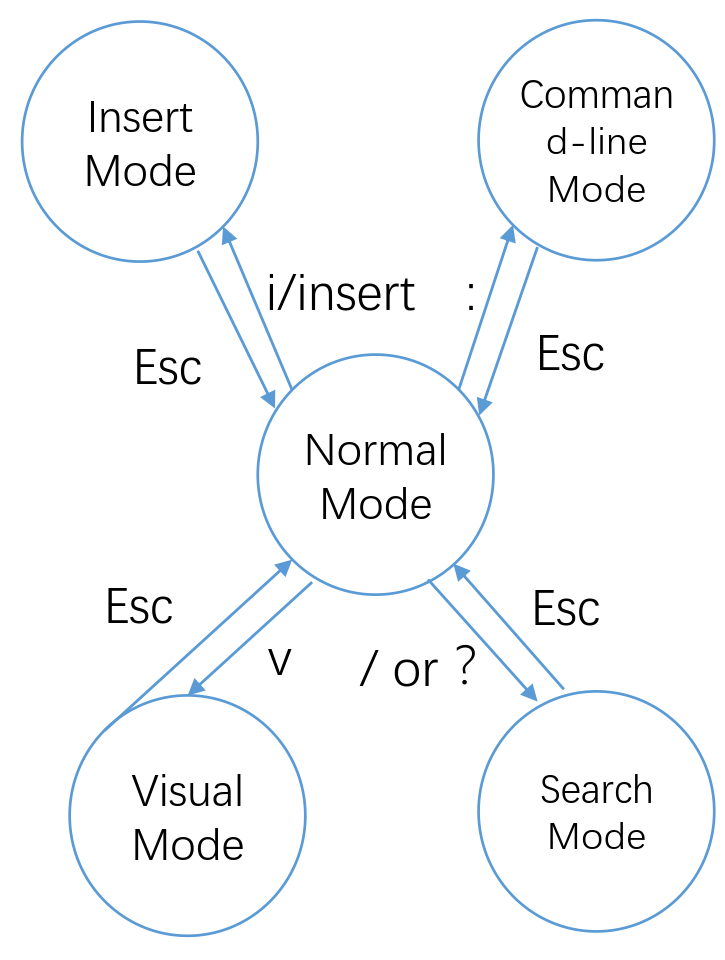
\includegraphics[width=5cm]{5.png}
    \caption{vim的工作模式}
\end{figure}

\subsubsection{各模式下的操作}
\begin{enumerate}[label=\arabic*.]
    \item \textbf{普通模式}:可使用上下左右键、\mintinline{bash}{Home}、\mintinline{bash}{End}、\mintinline{bash}{PageUp}、\mintinline{bash}{PageDown}、\mintinline{bash}{gg}、\mintinline{bash}{Shift + g}等键移动光标,\mintinline{bash}{yy}复制当前行,\mintinline{bash}{dd}剪切当前行,\mintinline{bash}{p}粘贴,\mintinline{bash}{u}撤销,\mintinline{bash}{Ctrl + r}恢复撤销操作。
    \item \textbf{插入模式}:按\mintinline{bash}{i}键或\mintinline{bash}{Insert}键进入,支持方向键等移动光标,按\mintinline{bash}{Insert}键可切换插入和替换模式。
    \item \textbf{查找模式}:按\mintinline{bash}{/}或\mintinline{bash}{?}键进入,输入查找字符串并回车查找,按\mintinline{bash}{n}键查找下一项,\mintinline{bash}{Shift + n}查找上一项。
    \item \textbf{命令模式}:按\mintinline{bash}{:}键进入,输入\mintinline{bash}{w}保存,\mintinline{bash}{q}退出,\mintinline{bash}{wq}保存并退出等命令。
    \item \textbf{可视模式}:按\mintinline{bash}{v}键进入,移动光标选择文本块,\mintinline{bash}{y}键复制,\mintinline{bash}{d}键剪切,普通模式下\mintinline{bash}{p}键粘贴。
\end{enumerate}

\subsection{GNU工具链}
\subsubsection{GNU工具链简介}
GNU工具链是一组开源编程工具,由GNU计划提供,包含用于编译、调试和构建软件的实用程序,如GCC(支持多种编程语言的编译器集合)、GNU Binutils(包括汇编器、连接器等)、GDB(调试程序的工具)、Make(用于构建和管理项目的工具,通过Makefile文件描述构建规则)。

\subsubsection{构建程序}
\begin{enumerate}[label=\arabic*.]
    \item \textbf{单个源文件}:可使用\mintinline{bash}{gcc main.c}编译并链接\mintinline{c}{main.c},默认生成\mintinline{bash}{a.out};也可使用\mintinline{bash}{gcc -o main main.c}指定生成文件名为\mintinline{bash}{main}。
    \item \textbf{多个源文件}:如编译\mintinline{c}{a.c}和\mintinline{c}{b.c},可使用\mintinline{bash}{gcc a.c b.c -o p}直接编译链接生成\mintinline{bash}{p}文件;也可先\mintinline{bash}{gcc –c a.c b.c}生成目标文件,再\mintinline{bash}{gcc –o p a.o b.o}链接生成\mintinline{bash}{p}文件。
\end{enumerate}

\subsubsection{增量编译}
只编译修改的文件再链接,可提高编译效率。如只编译\mintinline{c}{b.c},使用\mintinline{bash}{gcc –c b.c},再\mintinline{bash}{gcc –o p a.o b.o}链接。

\subsubsection{引用自定义头文件与链接第三方库}
引用自定义头文件时,使用\mintinline{bash}{-I}指定头文件搜索目录,如\mintinline{bash}{gcc –c a.c –Iinc}。链接第三方库时,使用\mintinline{bash}{-l}指定库名称,如\mintinline{bash}{gcc –o p a.o -lm}链接数学库;若库不在默认搜索路径,使用\mintinline{bash}{-L}指定路径。

\subsubsection{自动化编译}
\begin{enumerate}[label=\arabic*.]
    \item \textbf{编写shell脚本}:编写脚本可简化编译过程,但存在局限性,如处理复杂项目时脚本复杂、无法增量编译等。
    \item \textbf{使用Makefile}:在工程根目录创建Makefile文件,编写规则后使用\mintinline{bash}{make}命令编译。Makefile中可定义变量,如\mintinline{bash}{CC}(编译器)、\mintinline{bash}{CFLAGS}(编译选项)等,规则包含目标、依赖和命令,\mintinline{bash}{make}会根据依赖关系和时间戳确定编译操作。
\end{enumerate}

\subsubsection{在编译程序时增加调试信息}
编译时添加\mintinline{bash}{-g}选项,如\mintinline{bash}{CFLAGS = -Iinc -g},可使编译器在生成目标文件时包含调试信息,便于使用GDB调试程序,如设置断点、查看变量值等。


\subsection{代码版本管理}
\subsubsection{创建本地仓库与提交文件}
使用\mintinline{bash}{mkdir}创建本地工作目录,\mintinline{bash}{cd}进入目录,\mintinline{bash}{git init}创建空的本地仓库。创建文件后使用\mintinline{bash}{git add}将文件转换为staged状态,再用\mintinline{bash}{git commit}提交至版本库,提交时可编辑提交说明。
\begin{figure}[H]
    \centering
    \captionsetup{skip=4pt}
    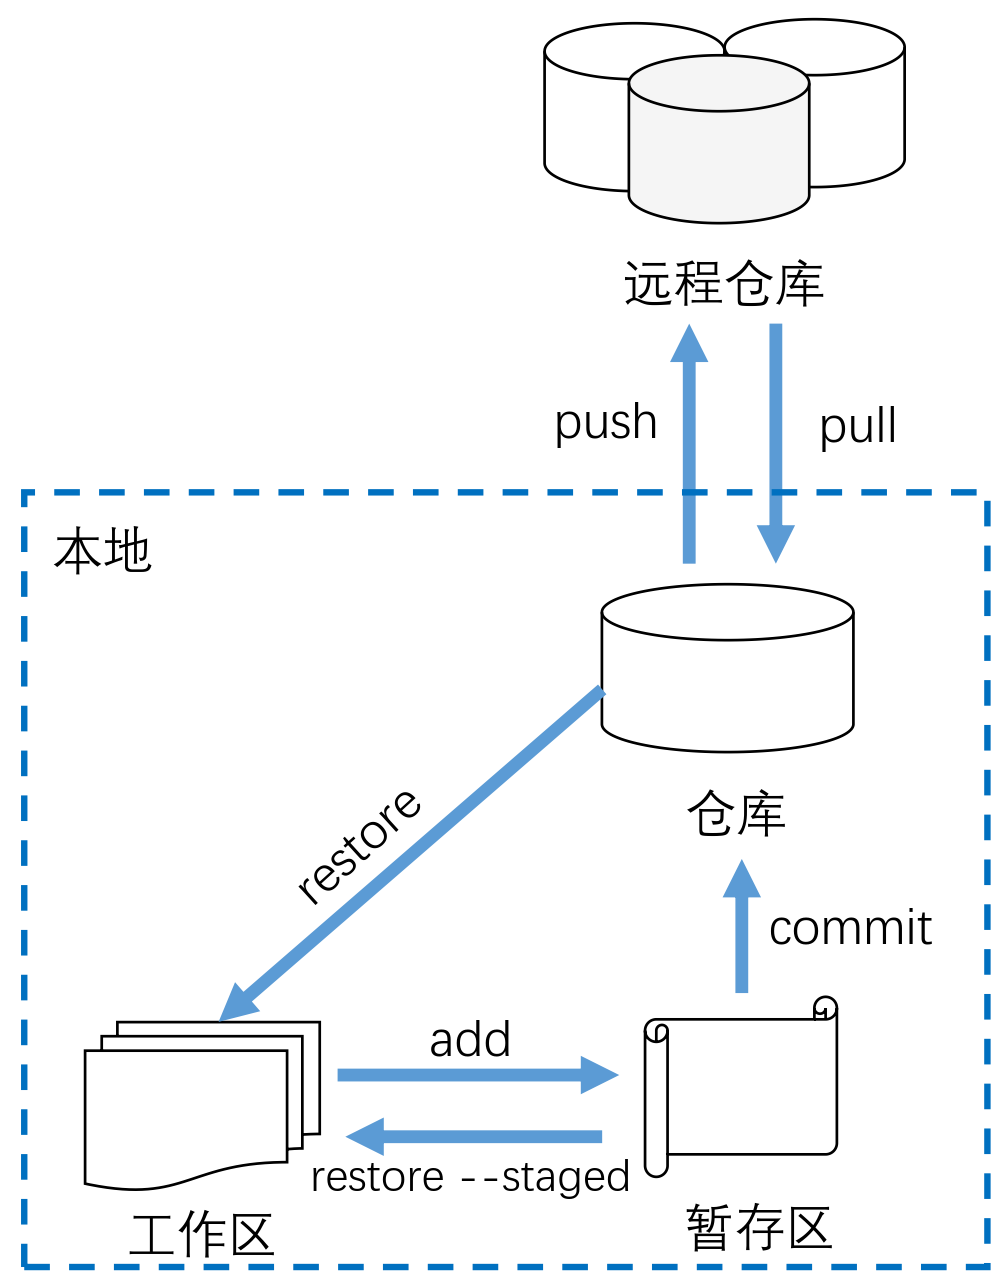
\includegraphics[width=5cm]{6.png}
    \caption{git示意图} 
\end{figure}

\subsubsection{查看提交日志与代码还原}
使用\mintinline{bash}{git log}命令可查看提交日志,包含提交记录标识、作者、日期和提交说明等信息。使用\mintinline{bash}{git restore}命令可进行代码还原,如\mintinline{bash}{git restore main.c}用最近一次提交覆盖工作区文件,也可指定提交记录标识还原。

\subsubsection{远程仓库操作}
使用\mintinline{bash}{git remote add origin 远程仓库地址}关联远程仓库,首次推送使用\mintinline{bash}{git push -u origin master},后续只需\mintinline{bash}{git push}。也可使用\mintinline{bash}{git clone}命令克隆远程仓库至本地。

